\section{Localizar novos parceiros}

\par Esta busca permite ao usuário encontrar novos parceiros para compor a sua rede de relacionamentos. Para realizar esta busca, utilizou-se a mesma consulta da funcionalidade anterior, acrescentando apenas o filtro para permitir a busca por nomes informado pelo usuário. O Código~\ref{list:consulta_novos_parceiros} apresenta a \textit{query} utilizada para realizar esta busca.

\begin{lstlisting} [style=custom_SQL,caption={[\textit{Query} para apresentar novos parceiros]{\textit{Query} para apresentar novos parceiros. \textbf{Fonte:} Elaborado pelos autores.}}, label=list:consulta_novos_parceiros] 	
MATCH (me:Person {email: 'andressa_faria18@hotmail.com'}), (users:Person),
(users)-[:WORKS_IN]->(company)<-[:WORKS_IN]-(me)
WHERE users.name =~ 'Edil.*'
AND users.typeOfAccount <> 'SERVICE_PROVIDER'
AND users <> me AND NOT((users)-[:PARTNER_OF]->(me)-[:PARTNER_OF]->(users))  
OPTIONAL MATCH 
	pMutualFriends=(me)-[:PARTNER_OF]->(another)-[:PARTNER_OF]->(me), 
	(users)-[:PARTNER_OF]->(another)-[:PARTNER_OF]->(users) 
RETURN DISTINCT({name: users.name, email: users.email, length: 1, 
photo: users.photo, mutualFriends: count(DISTINCT pMutualFriends)}) 
as partner ORDER BY partner.length, partner.mutualFriends DESC 
UNION ALL 
MATCH (me:Person {email: 'andressa_faria18@hotmail.com'}), (users:Person),
(users)-[:LIVES_IN]-(city)<-[:LIVES_IN]-(me)
WHERE users.name =~ 'Edil.*'
AND users.typeOfAccount <> 'SERVICE_PROVIDER' 
AND NOT((users)-[:WORKS_IN]->()<-[:WORKS_IN]-(me)) 
AND NOT((users)-[:PARTNER_OF]->(me)-[:PARTNER_OF]->(users)) 
OPTIONAL MATCH 
	pMutualFriends=(me)-[:PARTNER_OF]->(another)-[:PARTNER_OF]->(me), 
	(users)-[:PARTNER_OF]->(another)-[:PARTNER_OF]->(users) 
RETURN DISTINCT({name: users.name, email: users.email, length: 2, 
photo: users.photo, mutualFriends: count(DISTINCT pMutualFriends)})
as partner ORDER BY partner.length, partner.mutualFriends DESC
\end{lstlisting}

% Trocado de figura para listagem
%\begin{figure}[h!]
%	\centerline{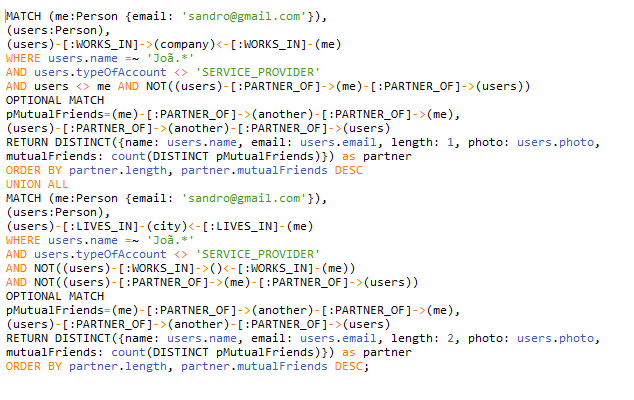
\includegraphics[scale=0.6]{./imagens/consulta-busca-novos-parceiros.png}}
%	\caption[\textit{Query} para apresentar novos parceiros.]
%	{\textit{Query} para apresentar novos parceiros \textbf{Fonte:} Elaborado pelos autores.}
%	\label{fig:consulta_novos_parceiros}
%\end{figure}

Essa consulta é muito parecida com a apresentada no Código~\ref{list:consulta_possiveis_parceiros}, porém, com uma diferença, pois, nesse caso há uma condição onde é levado em consideração o nome informado pelo usuário para localizar os possíveis novos parceiros.

\par A Figura~\ref{fig:busca_novos_parceiros} apresenta o resultado da busca por novos parceiros, contendo uma lista com as pessoas que atendam os requisitos pré estabelecidos na consulta.

\begin{figure}[h!]
	\centerline{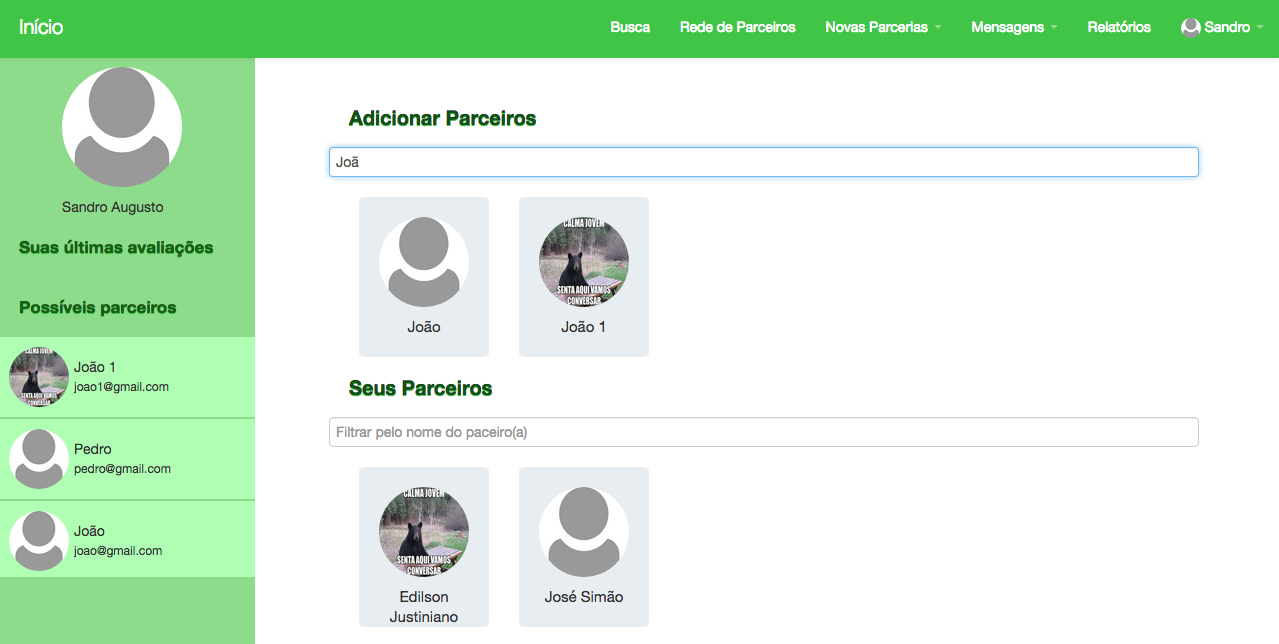
\includegraphics[scale=0.3]{./imagens/busca-novos-parceiros.png}}
	\caption[Funcionalidade que apresenta a busca por novos parceiros]
	{Funcionalidade que apresenta a busca por novos parceiros. \textbf{Fonte:} Elaborado pelos autores.}
	\label{fig:busca_novos_parceiros}
\end{figure}

\par  Esta funcionalidade permite então que o usuário localize novos parceiros, que são indicados por ele e não sugeridos pelo sistema, como acontece na funcionalidade anterior.